\section{Application: the stochastic Allen--Cahn field}
\label{sec:allen-cahn}

\begin{figure*}[t]
  \centering
  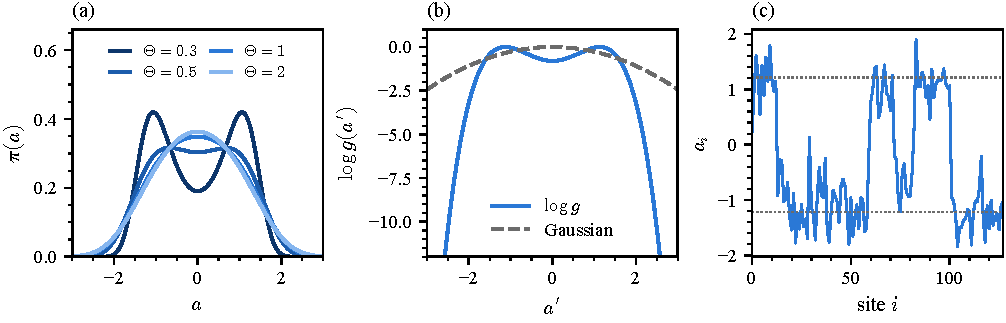
\includegraphics{fig_field}
  \caption{The Allen--Cahn chain. (a) Single-site law of the standardised field at the four temperatures.
  (b) The tilt $\log g$ of the kernel at $\Theta=0.3$ against the quadratic of the Gaussian chain with the same
  correlation. (c) One exact sample at $\Theta=0.3$; dotted lines mark the two wells.}
  \label{fig:field}
\end{figure*}

The stochastic Allen--Cahn equation\note{cite} describes a scalar field relaxing in a double-well potential,
\begin{equation}
  \partial_\tau\phi=\partial_x^2\phi-V'(\phi)+\sqrt{2\Theta}\,\eta,\qquad V(\phi)=\tfrac14(\phi^2-1)^2,
\end{equation}
with space-time white noise $\eta$ at temperature $\Theta$. On a lattice of spacing $h$ its stationary law is
\begin{equation}
  p(\phi)\propto\exp\Big(-\frac1\Theta\sum_i\Big[\frac{(\phi_{i+1}-\phi_i)^2}{2h}+hV(\phi_i)\Big]\Big),
\end{equation}
which is a nearest-neighbour chain, so everything above applies. Its kernel is a tilted random walk,
$K(a'\mid a)\propto\Normal(a';a,\gamma)\,g(a')$, for the standardised field $a=\phi/s$. Unlike the Laplace chain, the
\emph{shape} of the law of $a'$ depends on $a$: near zero it has two bumps, near a well it is one-sided. At low
temperature the field sits in one well or the other, with sharp kinks between them (\cref{fig:field}). We use four
temperatures, $\Theta=0.3$, $0.5$, $1$ and $2$, chains of $L=32$ sites, and a lattice spacing chosen so that
neighbouring sites have correlation $0.85$, as on the Laplace chain.
% src: outputs/E32/cells.json (rho1 = 0.848 at T0.3_h1, 0.850 at the iso cells)

\begin{table}[t]
  \caption{Allen--Cahn field: relative score error divided by that of the best linear denoiser, from $M=2048$
  training sequences, mean over 16 seeds. Parameters in brackets. Dashes: not run.}
  \label{tab:field}
  \centering
  \small
  \setlength{\tabcolsep}{4pt}
  \begin{tabular}{@{}lcccc@{}}
    \toprule
    $\Theta$ & 0.3 & 0.5 & 1 & 2\\
    \midrule
    site energy (5)          & 0.033 & 0.072 & 0.141 & 0.169\\
    tilted spline (25)       & 0.060 & 0.134 & 0.280 & 0.428\\
    log-linear 2-D (100)     & 0.184 & --    & 0.428 & --\\
    MDN (1{,}516)            & 0.228 & 0.422 & 0.738 & 0.838\\
    shift mixture (25)       & 1.004 & 1.004 & 1.014 & 1.021\\
    best network             & 0.484 & 1.174 & 2.157 & 3.044\\
    \bottomrule
  \end{tabular}
  % src: ~/Code/Thesis/jerome-call-2026-10-29-slide15.md (frozen E33 hpc_E33k/q/n, E43 hpc_E43a, floor hpc_E33o)
  % pending: neural energy kernel row (E55) and its U-Net comparison
\end{table}

\Cref{tab:field} compares kernel families with the best network (the better of a window CNN and a transformer, each
trained with two score-matching losses). Every family whose conditional law depends on $a$ beats the best network at
every temperature, including two that know nothing about the field: the log-linear kernel ($0.18$ against $0.48$ at
$\Theta=0.3$) and a mixture density network. The same holds with $M=128$ training sequences (\cref{app:field}).
% src: slide15.md M=128 table: every nonlinear family < best network in every cell
The shift mixture of \cref{sec:families} is no better than the linear denoiser. It does not collapse: all eight
components are used. But a shift kernel has a linear drift and the same innovation law at every $a$, so the best
member of the family is close to a Gaussian chain, and BP with a Gaussian kernel is linear. The family has to be able
to represent the data; a regulariser would not help.
% src: slide15.md: effective number of components exp H(pi) = 7.8 of 8 (median), max weight 0.18, fitted excess kurtosis -0.03 to -0.04

The data efficiency shows across sizes. With 128 sequences the site-energy kernel ($0.14$ at $\Theta=0.3$) is still
3.5 times better than the best network with 2048 ($0.48$).
% src: slide15.md point 4
Because the site energy has the form of the lattice action, it also returns the physical parameters: the temperature
comes out as $\hat\Theta=\hat\gamma s^2/h$, with seed means of $\hat\Theta/\Theta$ between $0.9995$ and $1.0068$ over
six cells, and the potential $V$ up to a constant.
% src: answers note Q8 (E33, six cells, 16 seeds)
\pending{E55: the neural energy kernel against a DDPM U-Net on the same cells.}
